% Dokumenttyp
\documentclass[a4paper,11pt,twoside,german]{article}

% Befehle für Seitenränder
\newcommand{\largeborder}{3cm}
\newcommand{\smallborder}{2cm}
\newcommand{\topborder}{1cm}
\newcommand{\bottomborder}{1cm}

\usepackage[
    left=\largeborder,
    right=\largeborder,
    top=\topborder,
    bottom=\bottomborder,
    includeheadfoot,
    ]{geometry}
    
% \textwidth 16cm
% \textheight 24cm
%  \topmargin -15mm
% \setlength{\oddsidemargin}{-5mm}
% \setlength{\evensidemargin}{5mm}


%%%%%%%%%%%%%%%%%%%%%%%%%%
%%% Benötigte Packages %%%
%%%%%%%%%%%%%%%%%%%%%%%%%%

%%% Sprache %%%
\usepackage[ngerman]{babel}    	% damit man deutsche Dinge tun kann
\usepackage{ziffer} % Deutsche Zahlen (kein Abstand hinterm Komma, Punkt als Tausendertrennzeichen, etc...)
\usepackage[utf8]{inputenc}   % damit Umlaute funktionieren
\usepackage[autostyle=true,german=quotes]{csquotes} % Anführungszeichen richtig machen
\usepackage{blindtext} % damit man sinnlosen Text produzieren kann

%%% Grafiken %%%
\usepackage{graphicx}    % damit man Bilder einbinden kann
% \usepackage{float}    	% damit Floats da sind, wo sie hingehören
\usepackage{floatrow}   % bessere float Organisation
\usepackage[font=footnotesize,labelfont=bf,skip=0pt]{caption} % Captions anpassen
\addtolength{\intextsep}{5mm} % mehr Platz um figures und tables
\usepackage{subcaption}


\usepackage{amsmath}    	% damit abgefahrene mathematische Dinge in equations gehen
\usepackage{enumitem}   % Damit Aufzählungen hübscher sind
\usepackage{ifthen}     % Damit man if-else-Strukturen machen kann

\setlength{\parindent}{0pt} % Keine Absatzeinrückung
\usepackage{setspace} % Zeilenabstände machen können
\linespread{1.1} % Zeilenabstand definieren
\newcommand{\absatz}{\smallbreak} % Standardmäßig \absatz zur Trennung von Absätzen verwendet und hier das Kommando anpassen
%\renewcommand{\familydefault}{\sfdefault} % Serifenlose Schrift

%%% Links und Verweise %%%
\usepackage[breaklinks]{hyperref} % Damit Links funktionieren
\hypersetup{colorlinks=false,pdfborder={0 0 0}} % Damit die hässlichen Kästen um Links weg sind


%%% Bibliographie %%%
\usepackage[authoryear,round]{natbib} % Der Stil der LiteraturVERWEISE im Text
\bibliographystyle{dcu-german-spec} % Der Stil des LiteraturVERZEICHNISSES
%\bibliographystyle{dcu} % Der Stil des LiteraturVERZEICHNISSES


% Makro für Bibliographie
\newcommand{\literaturverzeichnis}[1]{
    \renewcommand{\harvardand}{und} % ein UND statt AND bei mehreren Autoren
    \bibliography{#1}
    }

\usepackage[nottoc,notlot,notlof]{tocbibind} % damit das Literaturverzeichnis im Inhaltsverzeichnis auftaucht, aber NICHT nummeriert wird
% \usepackage[nottoc,numbib]{tocbibind} % damit das Literaturverzeichnis nummeriert wird und im Inhaltsverzeichnis auftaucht


% Commands to place things on a left or right side
% Put this before something you want to place either right (onto the NEXT EVEN page) or left (onto the NEXT ODD page)
\newcommand{\emptypage}{\newpage\leavevmode\thispagestyle{empty}\newpage}
\newcommand{\fillwithemptypagestillevenside}{\ifthenelse{\isodd{\thepage}}{\emptypage}{}}
\newcommand{\fillwithemptypagestilloddside}{\ifthenelse{\isodd{\thepage}}{}{\emptypage}}

\newcommand{\breaktoevenside}{\ifthenelse{\isodd{\thepage}}{\newpage}{}}
\newcommand{\breaktooddside}{\ifthenelse{\isodd{\thepage}}{}{\newpage}}

% Metadaten
\usepackage{titling}
\title{LEX extended abstract}
\author{
    Büchau, Yann Georg \\
    \small{\texttt{64\,36\,211}}
    \and
    Finn, Tobias Sebastian \\
    \small{\texttt{00\,00\,000}}
    \and 
    Schaper, Maximilian \\
    \small{\texttt{00\,00\,000}}
    }
%%%%%%%%%%%%%%%%%%%%%%%%%%%%%%%%%%%%%%%%%%
\begin{document}
\raggedbottom


%%%%%%%%%%%%%%%%%%
%%% Titelseite %%%
%%%%%%%%%%%%%%%%%%

\hypersetup{pageanchor=false}
\makeatletter
\begin{titlepage}

%\newgeometry{
%    left=\smallborder,
%    right=\smallborder,
%    top=\topborder,
%    bottom=\bottomborder,
%    includeheadfoot,
%    }


\vspace*{\fill}
\begin{center}
\Large{\textbf{Lehrexkursion Fehmarn}}\\
\large{29.08.2016 - 09.09.2016}\\
\vspace{5mm}
\Large{\textbf{Arbeitsgruppe\\Wolkenkamera Stereo}}\\
\vspace{1cm}

% authors
\begin{large}
\begin{tabular}{ccc}
Büchau, Yann Georg & Finn, Tobias Sebastian & Schaper, Maximilian \\
\small{\texttt{64\,36\,211}} & 
\small{\texttt{00\,00\,000}} &
\small{\texttt{00\,00\,000}}
\end{tabular}
\end{large}

\vspace{1cm}
\large{Meteorologisches Institut}\\
\large{Universität Hamburg}\\
\vspace{1cm}
\large{{\today}}
\end{center}
\vspace*{\fill}

\clearpage
% \restoregeometry


\end{titlepage}
\makeatother
\hypersetup{pageanchor=true}

\newpage

%%%%%%%%%%%%%%%%%%%%%%%%%%
%%% Inhaltsverzeichnis %%%
%%%%%%%%%%%%%%%%%%%%%%%%%%
\clearpage
\setcounter{page}{1} % Page counting begins here!

\tableofcontents % Inhaltsverzeichnis
\vspace*{\fill}

%%%%%%%%%%%%%%%%%%%%%%%%%%%%%
%%% Abbildungsverzeichnis %%%
%%%%%%%%%%%%%%%%%%%%%%%%%%%%%
\listoftables % Abbildungsverzeichnis

\listoffigures % Abbildungsverzeichnis

\newpage


%%%%%%%%%%%%%%%%%%
%%% Motivation %%%
%%%%%%%%%%%%%%%%%%
\section{Motivation}

Ceilometer sind teuer, Kameras sind billig und vielseitig (Bedeckungsgrad,
Höhenwind, Wettergeschehen, etc...).  Es lohnt sich daher die Untersuchung,
inwiefern die Wolkenhöhe auch mit Kameras bestimmt werden kann.
\absatz
\blindtext[1]

%\newpage

%%%%%%%%%%%%%%
%%% Geräte %%%
%%%%%%%%%%%%%%
\section{Geräte}

Die verwendeten zwei Kameramodelle haben beide die Bezeichnung VIVOTEK FE8174V.
Metadaten sind in der Tabelle \ref{TabelleKameraMeta} zu finden.
Zum genauen Verstännis sei \cite{2016ingo} empfohlen.
\absatz

\begin{table}[!h]
\begin{center}
\caption{Metadaten der verwendeten Kameras}
\label{TabelleKameraMeta}
\absatz
\begin{tabular}{|c|c|c|}
\hline
\textbf{Kamera} & \textbf{GPS Position} & \textbf{Höhe über N.N.[m]} \\\hline
\textbf{Zaun}   & $54,4947^\circ\,\mathrm{N}$ \, $11,2408^\circ\,\mathrm{O}$ &
9                \\\hline
\textbf{Acker}   & $54,4959^\circ\,\mathrm{N}$ \, $11,2377^\circ\,\mathrm{O}$ &
0                \\\hline
\end{tabular}
\vspace{-0.5cm}
\end{center}
\end{table}

\blindtext

%\newpage % Neue Seite 

%%%%%%%%%%%%%%%%%%%
%%% Kalibration %%%
%%%%%%%%%%%%%%%%%%%
\section{Kalibration}

Grundlegend für die hier angewendete Triangulationsmethode ist die Kenntnis des
Azimuth- und Elevationswinkels in jedem Bildpunkt. Dazu ist eine Kalibration der
verwendeten Kameras erforderlich, mit der sowohl die radiale Projektion der
Kameralinse als auch die Drehungseffekte durch ungenaues Aufstellen der Kamera
quantifiziert werden können. Für eine derartige Kalibration sind Raumpunkte
nötig, deren Positionen sowohl auf dem Bild als auch in der Realität bekannt
sind. Es bietet sich hierfür die Sonne an, deren realer Azimuth- und
Elevationswinkel zu jedem Zeitpunkt berechenbar sind.
\absatz
Bedeckt man die Kamera an einem nahezu wolkenlosen Tag mit Goldfolie und
verringert die Helligkeitsempfindlichkeit der Kamera, erscheint die Sonne als
einziger heller Fleck auf dem ansonsten dunklen Bild (Abbildung \ref{FIGFolie}).
Das ermöglicht die programmatische Bestimmung der Sonnenposition auf dem Bild.
\absatz
Mit einer parameterbasierten Projektion, die Bildkoordinaten in reale
Koordinaten umrechnet, lassen sich durch Optimierung die optimalen Parameter
bestimmen, mit denen die Kalibration gut ist.
Die Kalibratoin ist dann ein Optimierungsproblem.
Dazu werden alle auf dem Bild gefundenen Sonnenpositionen auf eine
Einheitssphäre im realen Koordinatensystem projiziert. Der mittlere
quadratische Abstand zu den tatsächlichen Sonnenpositionen auf der
Einheitssphäre ist die zu optimierende Kostenfunktion in Abhängigkeit der
gewählten Projetionsparameter.
\absatz
Die Projektion funktioniert wie in (Abbildung \ref{FIGProjektion}).

\begin{figure}[!h]
\begin{center}
\begin{floatrow}
\ffigbox{
    \caption[Sonnenbahn auf mit Goldfolie bedeckten Kamera]{
    Zusammenstellung ausgewählter Aufnahmen der mit Goldfolie bedeckten Kamera
    \enquote{Zaun} bei einer groben Ausrichtung der optischen Achse (Bildmitte) (a) in
    den Zenith und (b) in die Mittagssonne.
    }
    \label{FIGFolie}
}{
    \begin{tabular}{cc}
        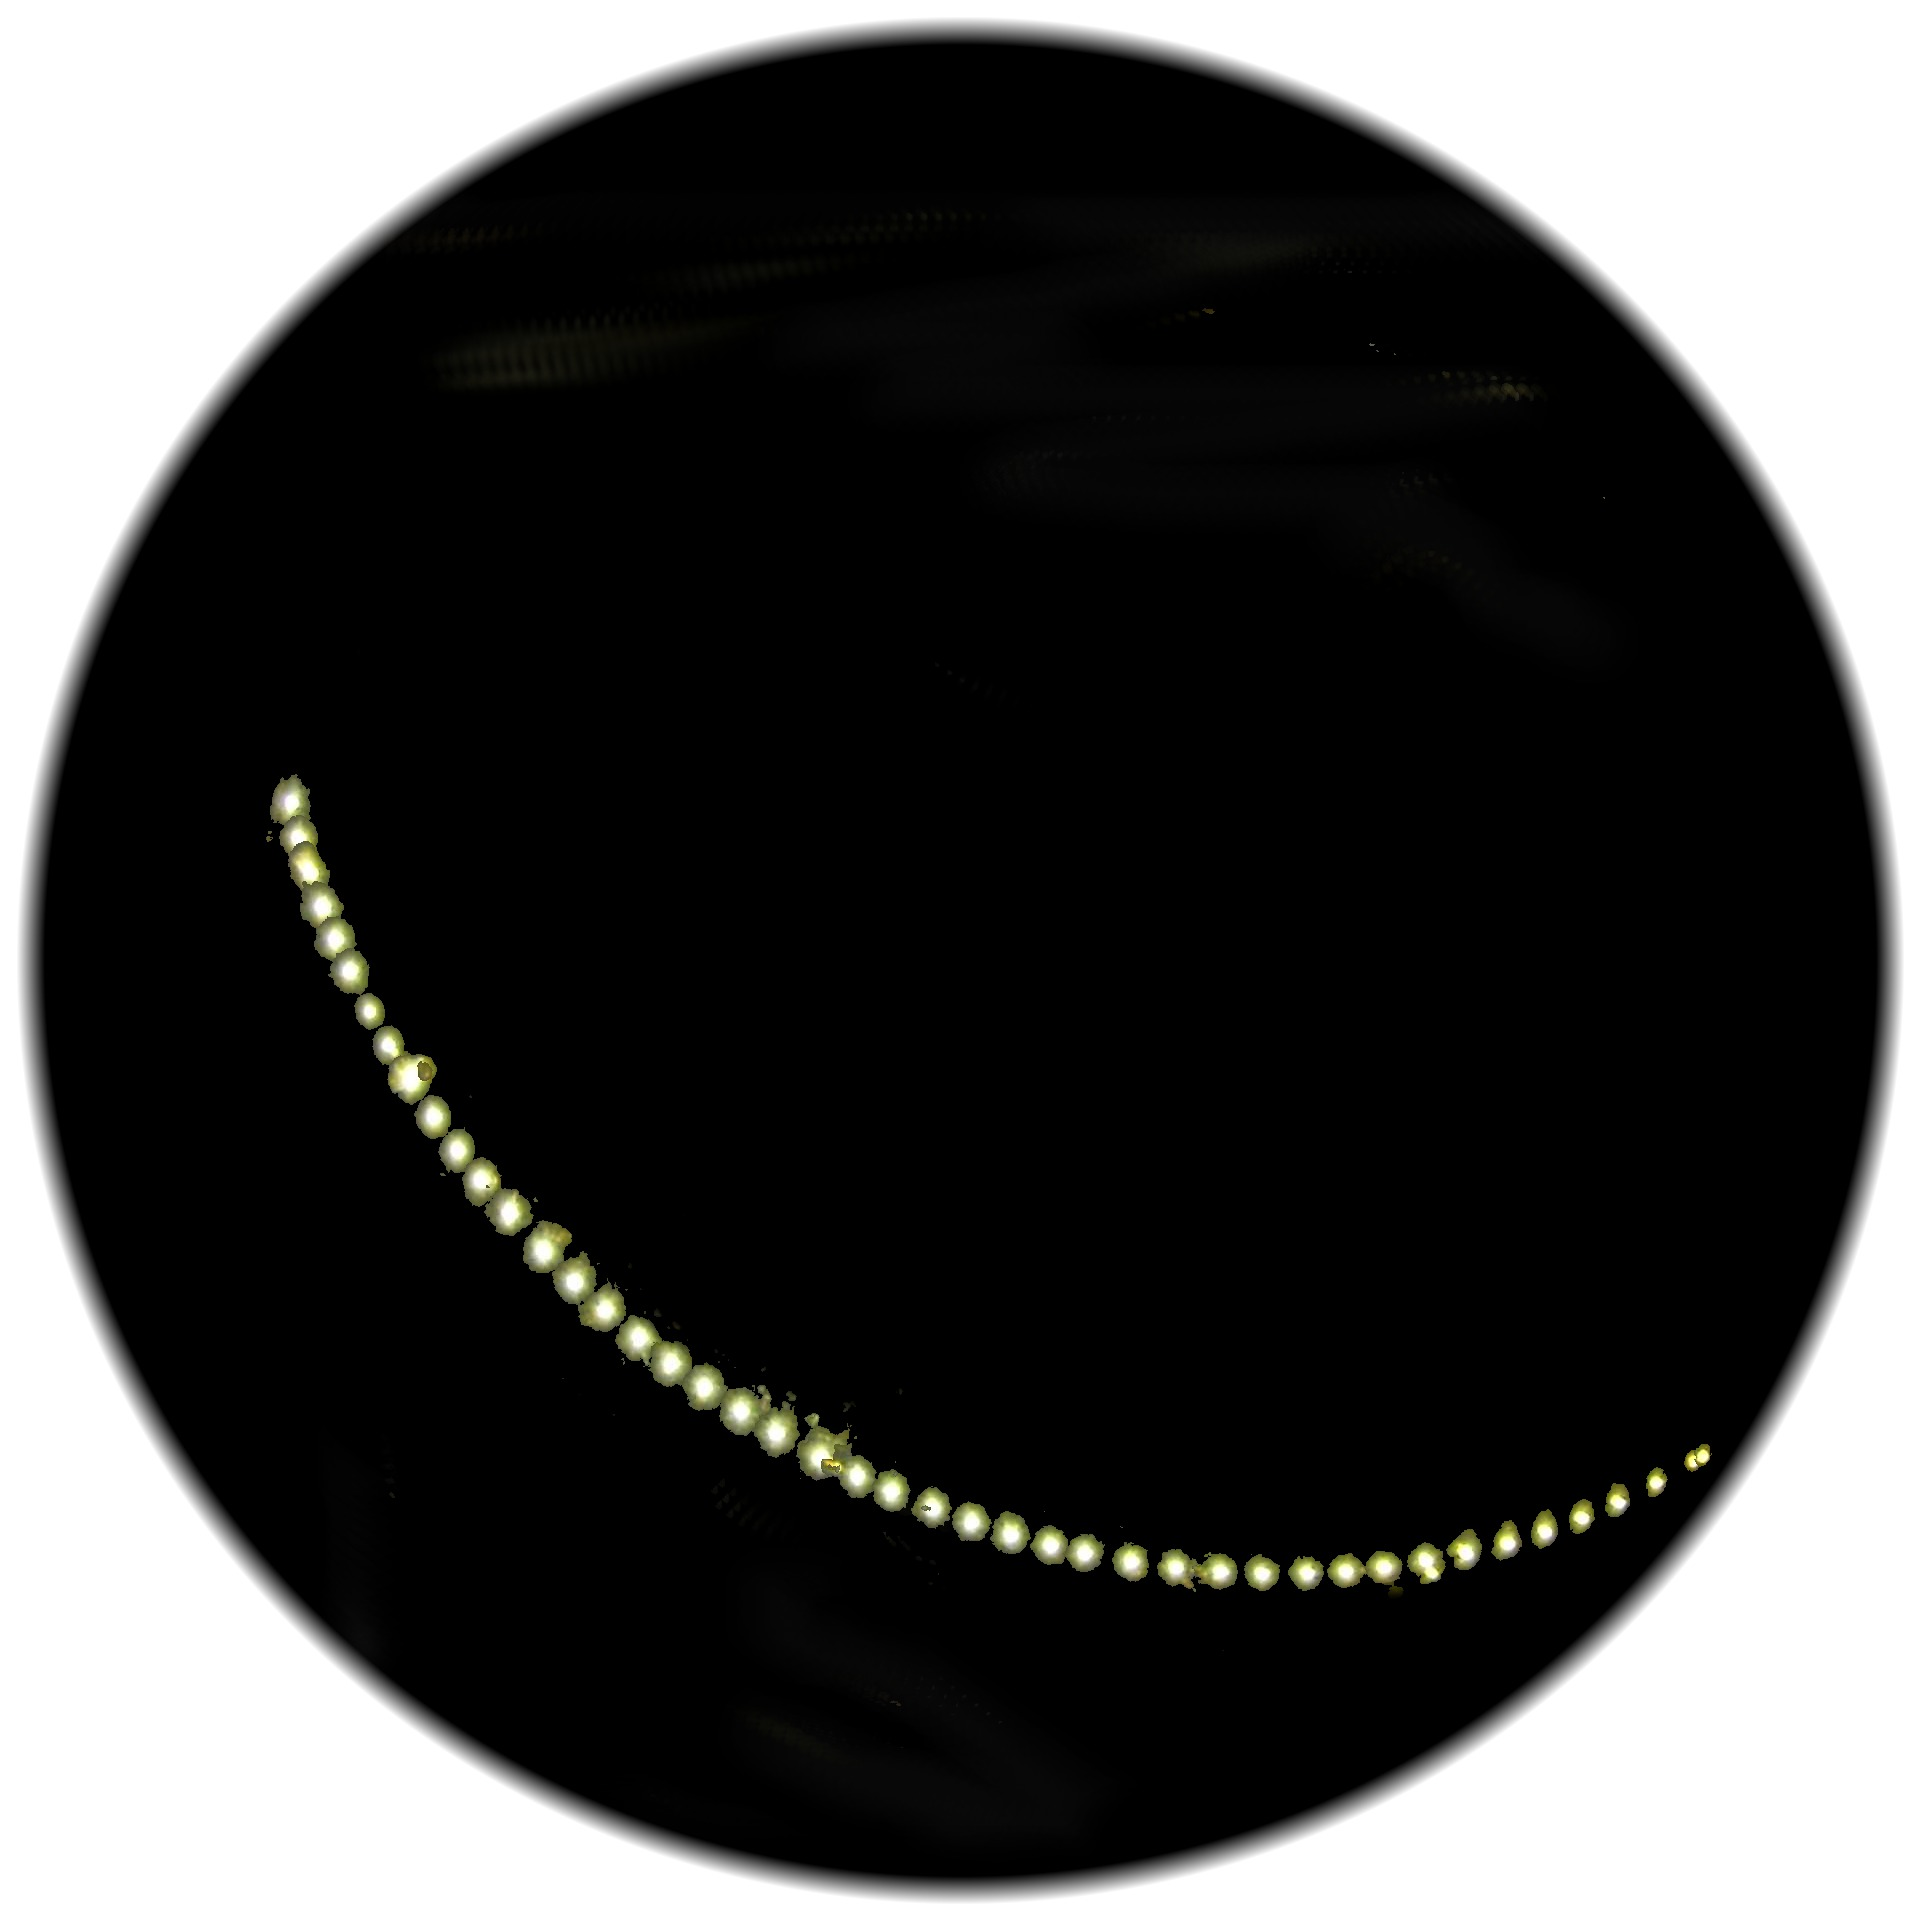
\includegraphics[width=0.22\textwidth]{media/cam3_straight_gold.jpg} &
        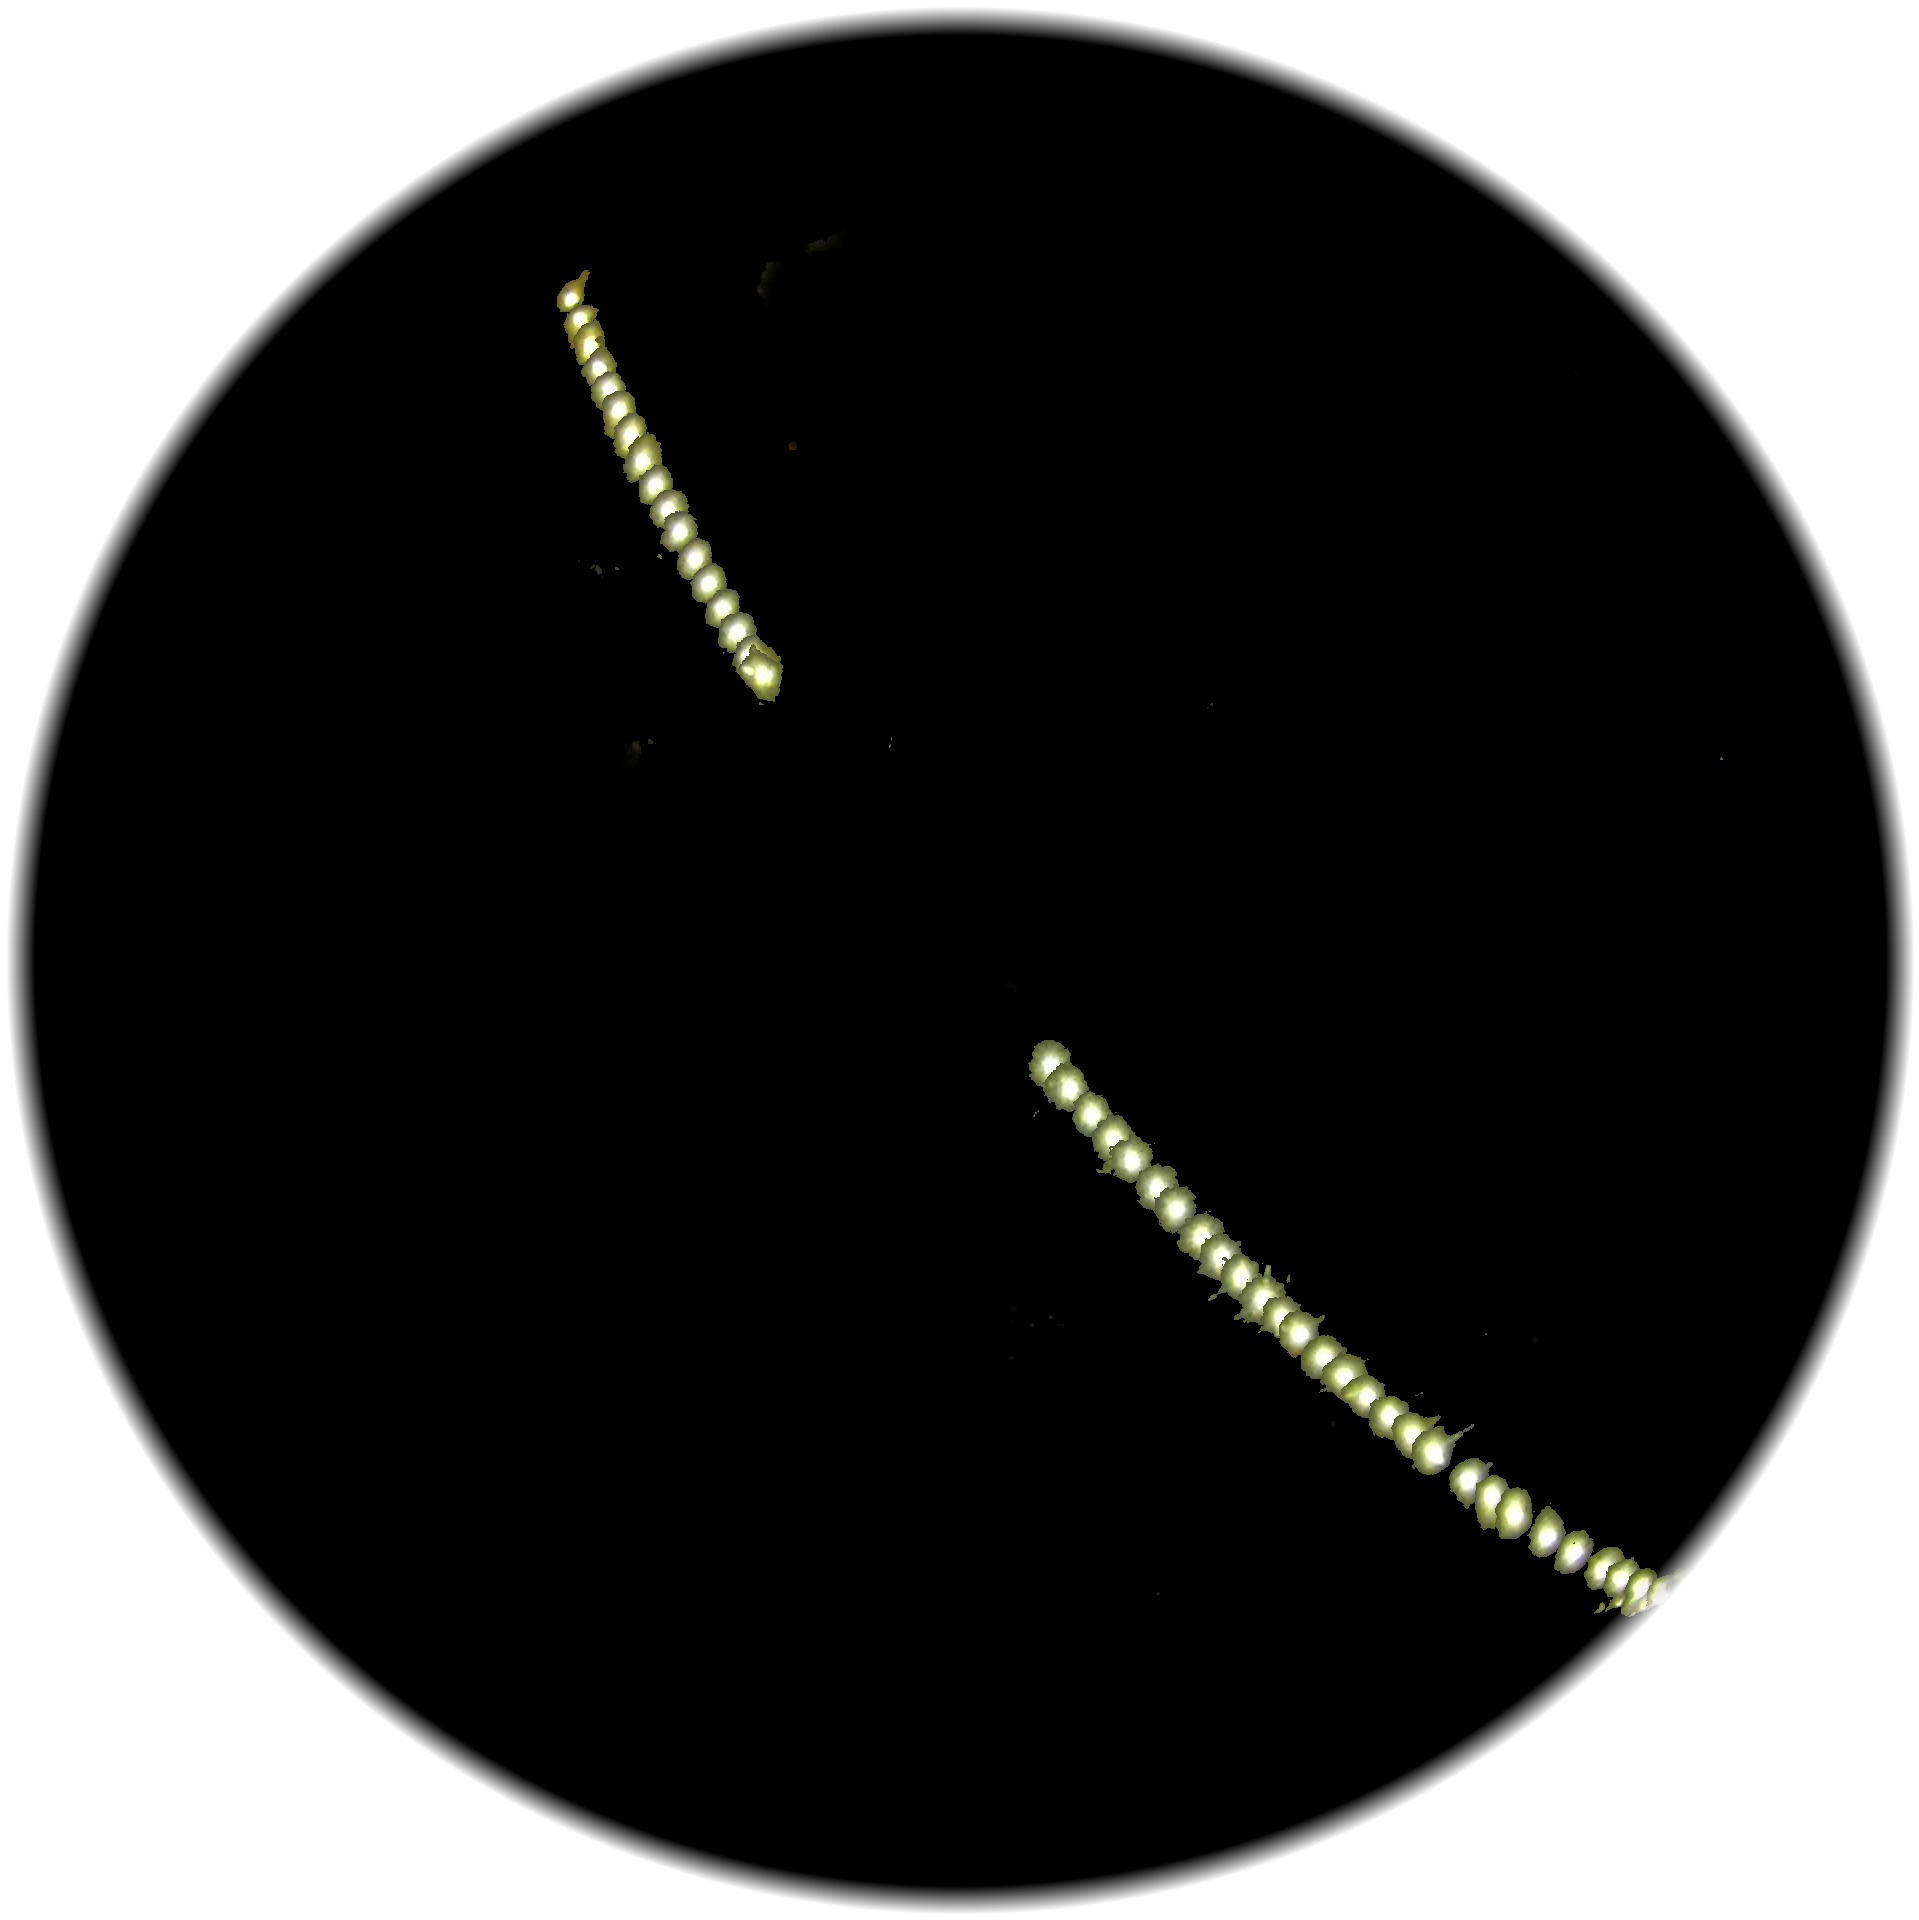
\includegraphics[width=0.22\textwidth]{media/cam3_proj_gold.jpg} \\
        (a) & (b) \\
    \end{tabular}
    }
    
\ffigbox{
    \caption[Projektion von Bildkoordinaten zu realen Koordinaten]{Projektion
    von Bildkoordinaten zu realen Koordinaten: (1) Sonne auf dem Bild (2)
    Elevation wird aus Radialprojektion angenährt (3)\,-\,(5) Drehung im Raum
    durch Euler-Winkel.  Die Punkte\ (2)\,-\,(5) befinden sich auf der
    Einheitsphäre.}
    \label{FIGProjektion}
}{
    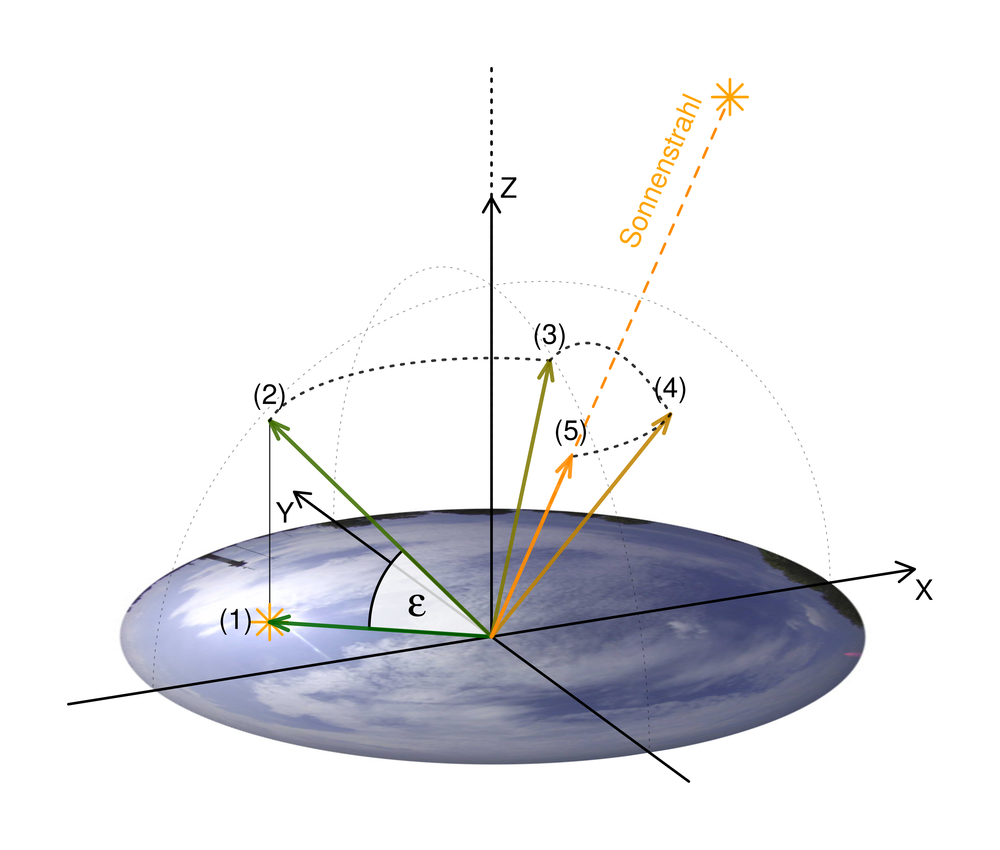
\includegraphics[width=0.49\textwidth]{media/calibration-chart.png}
}
\end{floatrow}
\end{center}
\end{figure}

%\newpage

%%%%%%%%%%%%%%%%%%%%%%%
%%% Wolkenerkennung %%%
%%%%%%%%%%%%%%%%%%%%%%%
\section{Wolkenerkennung}

Wolkenerkennung.
Machste halt k-Means...
\blindtext

%%%%%%%%%%%%%%%%%%%%%%%%
%%% Wolkenklustering %%%
%%%%%%%%%%%%%%%%%%%%%%%%
\subsection{Wolkenklusterung}

\blindtext[3]



%%%%%%%%%%%%%%%%%%%%%%
%%% Wolkenmatching %%%
%%%%%%%%%%%%%%%%%%%%%%
\subsection{Wolkenwiedererkennung}

Wolkenwiedererkennung.
\blindtext[3]


%\newpage


%%%%%%%%%%%%%%%%%%%%%%%
%%% Höhenbestimmung %%%
%%%%%%%%%%%%%%%%%%%%%%%
\section{Wolkenpositionierung}

Doppelanschnitt.
\blindtext[2]

%\newpage

%%%%%%%%%%%%%%%%%%%
%%% Validierung %%%
%%%%%%%%%%%%%%%%%%%
\section{Validierung}

Drachen und Ceilometer.
\blindtext[3]


%\newpage


%%%%%%%%%%%%%
%%% Fazit %%%
%%%%%%%%%%%%%
\section{Fazit}

Zusammenfassung.
\blindtext[3]

%\newpage % Neue Seite

%%%%%%%%%%%%%%%%%%%%%%%%%%%%
%%% Literaturverzeichnis %%%
%%%%%%%%%%%%%%%%%%%%%%%%%%%%
\literaturverzeichnis{bibliography.bib} % 



\end{document}
